\section{Network Designs for Disaggregation}
\label{sec:existing}

In this section, we explore whether existing network designs can meet the requirements identified in \S\ref{sec:requirements}, for the workloads from \S\ref{sec:workloads}. 
We start by describing our methodology (\S\ref{ssec:ssmethod}), then evaluate the network-level performance of a suite of network designs for \dis traffic workloads (\S\ref{ssec:nlp}), and finally 
evaluate how these designs impact application performance (\S\ref{ssec:alp}). 

%
\subsection{Methodology}
\label{ssec:ssmethod}

We evaluate the use of existing network designs for \dis in two steps.
First, we evaluate how existing network designs fare under \dis traffic workloads. 
For this, we consider a suite of state-of-the-art network designs and use simulation to evaluate their network-layer performance (flow completion time) for the workloads generated from \S\ref{sec:workloads}.
We then return to our real-world applications (Table~\ref{tab:workloads}) and once again 
emulate disaggregation by injecting latencies for page misses. 
However, now we inject the flow completion times obtained from our best-performing network design (as opposed to the constant latencies from \S\ref{sec:requirements}). 
This effectively `closes the loop', allowing us to evaluate the impact of disaggregation on 
application-level performance for realistic network designs and conditions. 

%
\begin{figure*}
  \centering
    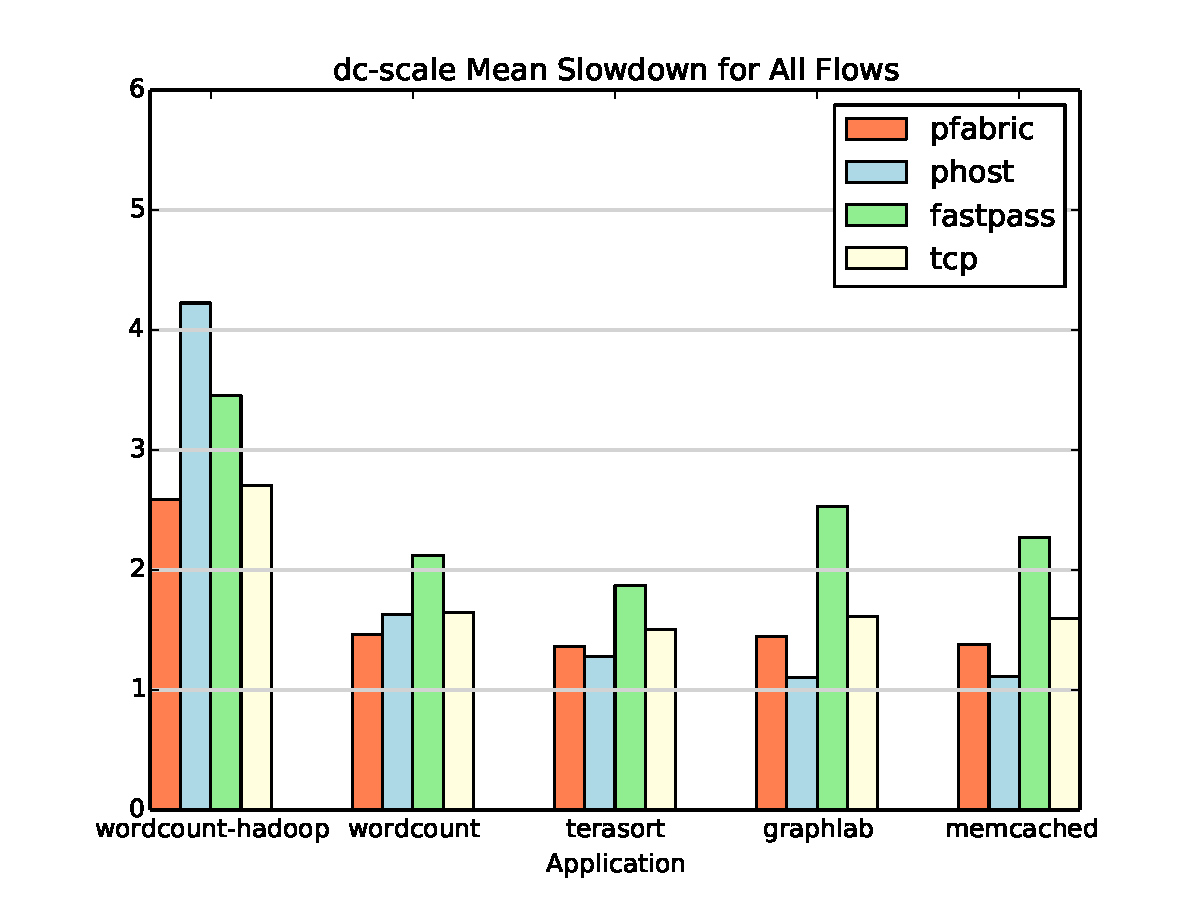
\includegraphics[width = 2in]{img/fig12_dc-scale_slowdowns} 
    \subfigure{
    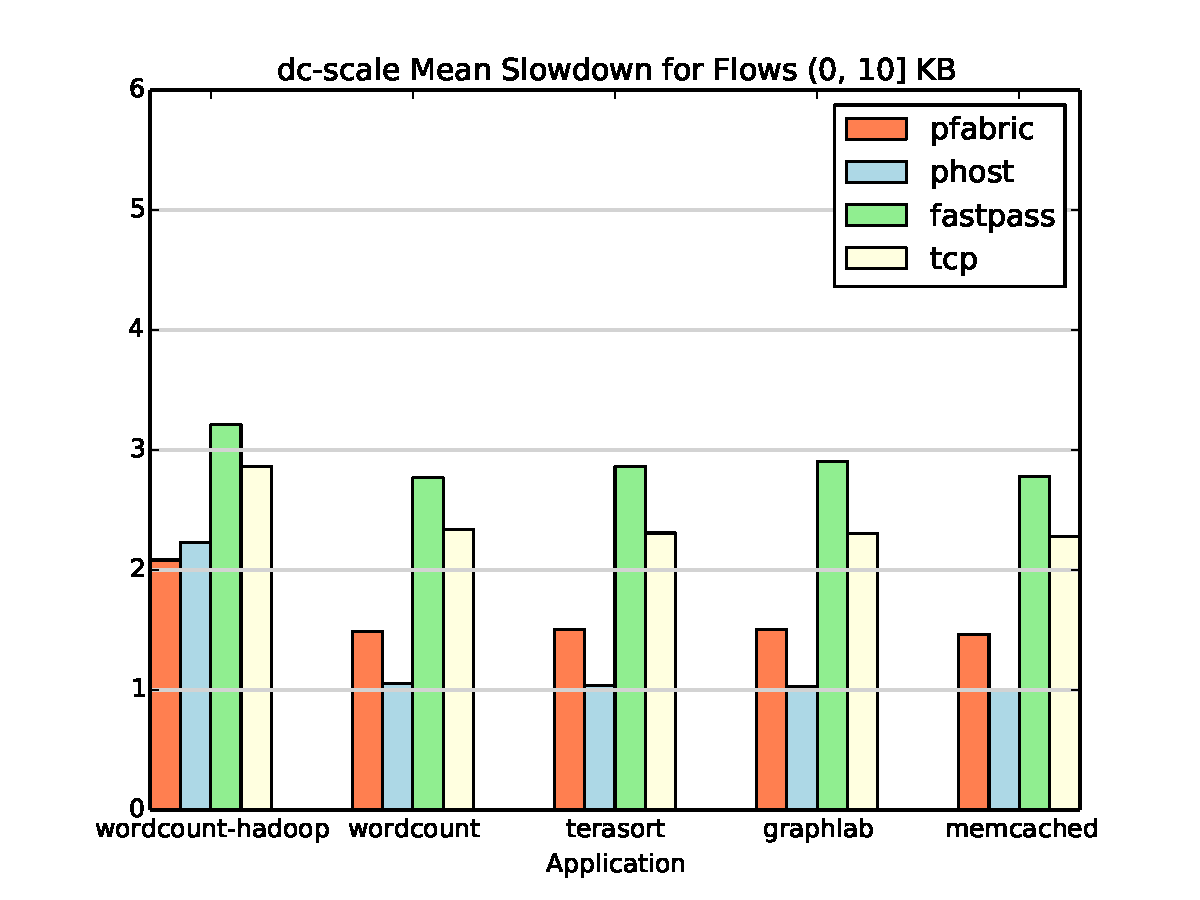
\includegraphics[width=2in]{img/fig12_dc-scale_slowdowns_small}
    }
    \subfigure{
    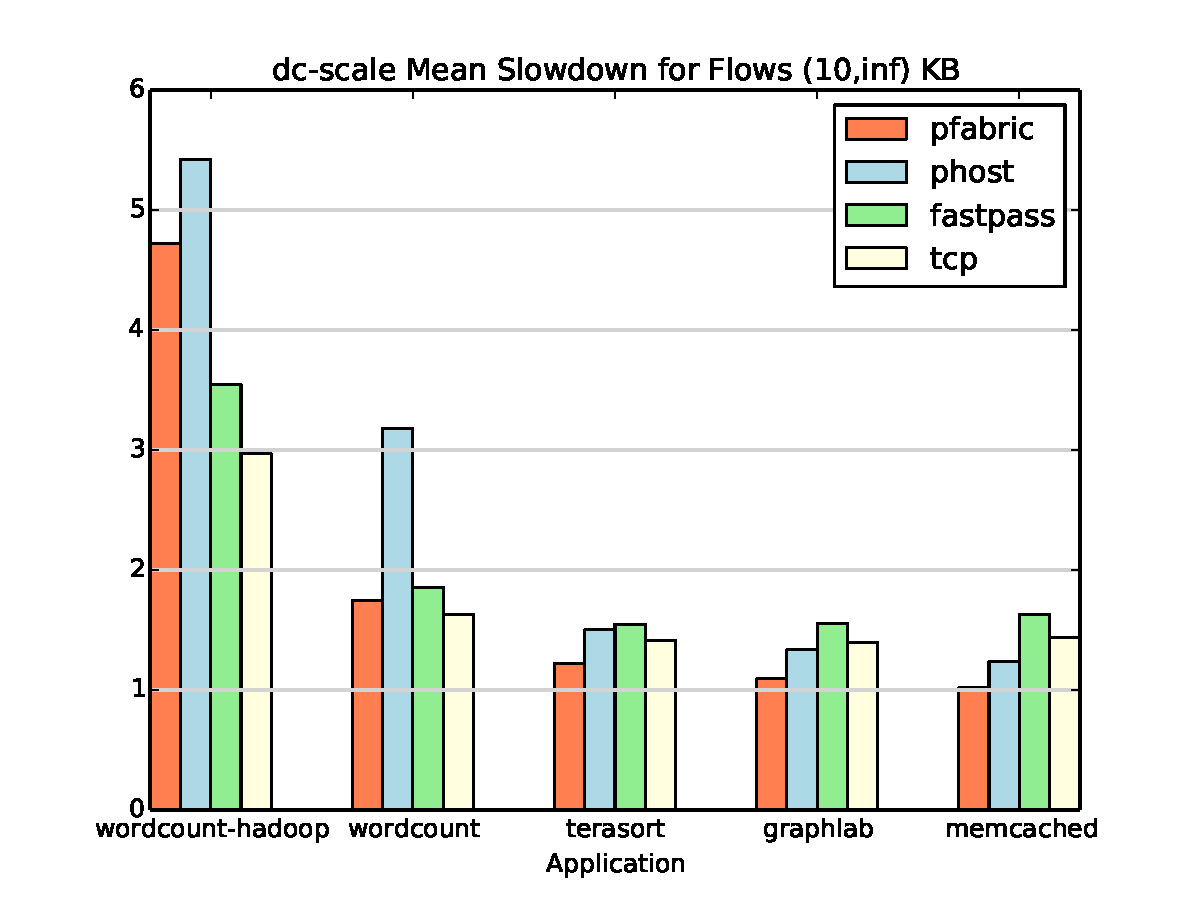
\includegraphics[width=2in]{img/fig12_dc-scale_slowdowns_big}
    }
  \caption{\small{The mean slowdown for pFabric, pHost, fastpass, and TCP for each of the five applications at datacenter-scale: (left) overall; (center) short flows only; (right) long flows.}}
  \label{fig:phostp-ds}
\end{figure*}
%

%
\begin{figure*}
  \centering
    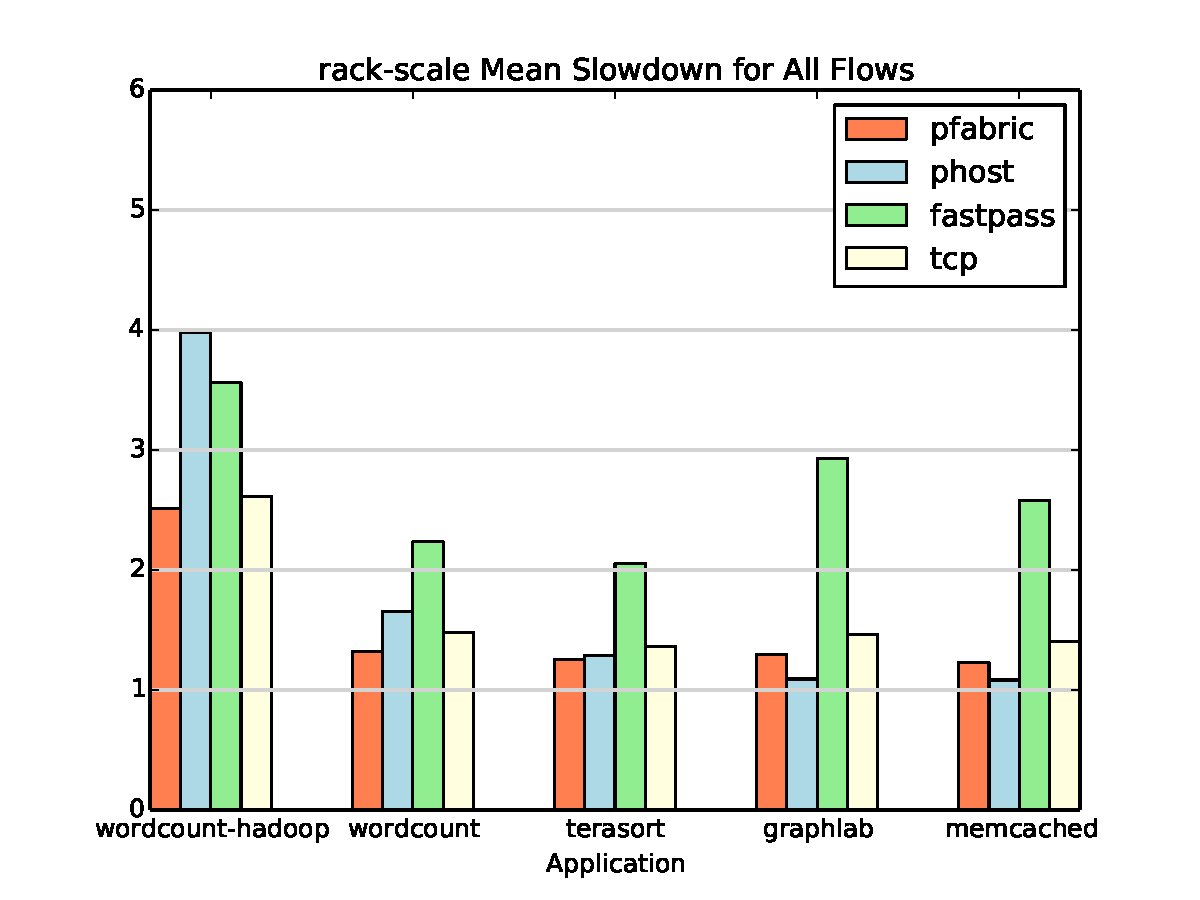
\includegraphics[width = 2in]{img/fig12_rack-scale_slowdowns} 
    \subfigure{
    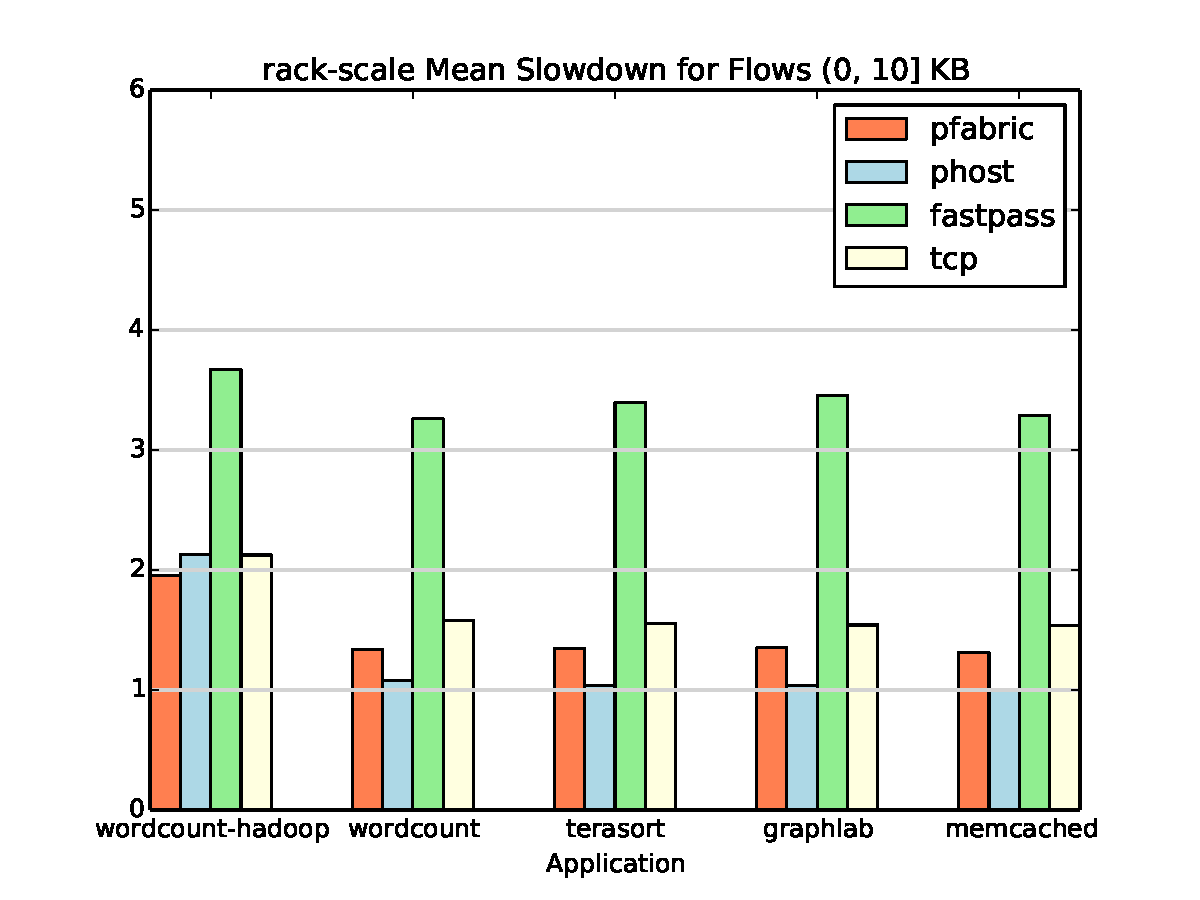
\includegraphics[width=2in]{img/fig12_rack-scale_slowdowns_small}
    }
    \subfigure{
    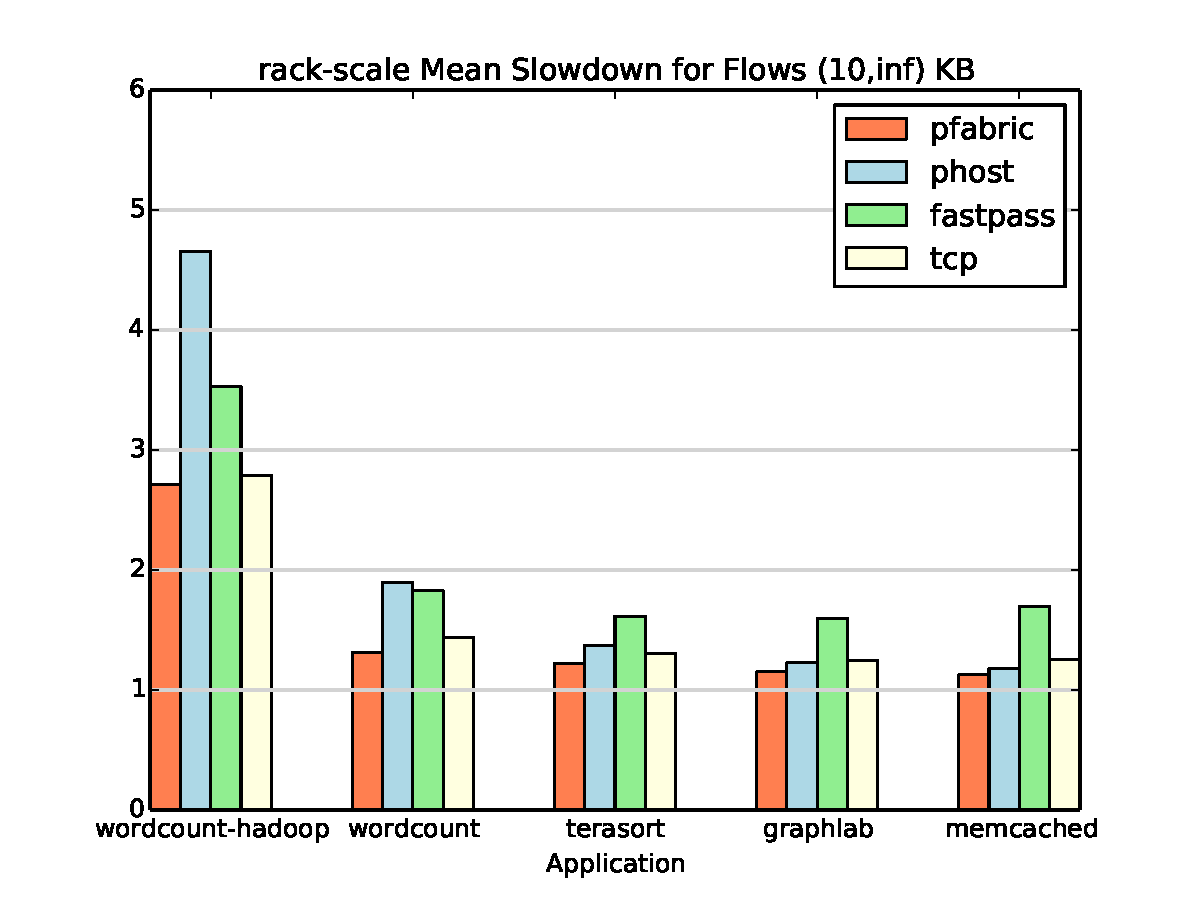
\includegraphics[width=2in]{img/fig12_rack-scale_slowdowns_big}
    }
  \caption{\small{The mean slowdown for pFabric, pHost, Fastpass, and TCP for each of the five applications at rack-scale: (left) overall; (center) short flows only; (right) long flows.}}
  \label{fig:phostp-rs}
\end{figure*}
%
For all the simulations in this section, we use the same setup as prior work on datacenter transport designs~\cite{pfabric, phost}. We simulate a $144$-node full bisection bandwidth Clos topology, $0.2$us of latency per hop, and $36$KB buffers per port; our only change is to use $40$Gbps link speeds at the edge as per our discussion in~\S\ref{sec:requirements}. We evaluate the following three protocols. In each case, we set protocol-specific parameters to the values that we found (through experimentation) yielded the best performance for that protocol.

\begin{enumerate}
\item \paragraphb{pFabric} The pFabric protocol~\cite{pfabric} achieves near-optimal flow completion times by approximating the behavior of shortest-job-first scheduling in a network context. pFabric uses specialized switch hardware to support scheduling that prioritizes flows with a smaller remaining flow size. We set pFabric to have an initial congestion window of 2 packets and a retransmission timeout of $45$us.
%
\item \paragraphb{pHost} pHost~\cite{phost} answers the question of how close a protocol can get to pFabric's performance by scheduling only at the end hosts. This allows the use of commodity switches as well as flexibility in policy selection. We set pHost to have a free token limit of 8 packets and a retransmission timeout of $9.5$us.
%; we obtained these parameters from pHost's implementation.
%
\item \paragraphb{Fastpass} Fastpass~\cite{fastpass} introduces a centralized scheduler that schedules  every packet. We implement Fastpass's scheduling algorithm in our simulator and optimistically assume that the scheduler's decision logic itself incurs no overhead (i.e., takes zero time) and hence we only consider the latency and bandwidth overhead of contacting the central scheduler. The implementation of this centralized arbiter is discussed in detail in previous work~\cite{phost}. We set the Fastpass epoch size to be 8 packets.%, obtained from the Fastpass paper.
%
\end{enumerate}

%There were multiple challenges in performing the above evaluations that we encountered.

\paragraphb{Traffic Generation}
As mentioned above, the disaggregated cluster we simulate includes $144$ nodes 
with 55 CPU, 55 memory and 34 disk blades. 
Each CPU blade is associated with 12 remote memory and disk blades (i.e., the `VM' abstraction in our simulation comprises one CPU whose memory and disk address space 
is spread across 12 remote blades). 
We generate traffic in this topology as follows. From our workload traces obtained in \S\ref{sec:workloads}, we generate CDFs representing the various distributions of flow 
sizes and flow inter-arrival times for each CPU blade. Each CPU blade draws from these distributions to generate flows directed at its associated 12 remote memory and disk blades. In addition, a CPU blade in our simulation generates 3x the load it does 
in our experiments from \S\ref{sec:workloads}; a single node in the original (non-disaggregated) cluster is replaced by three nodes in the disaggregated cluster and hence we do this 3x scale-up to maintain a comparable level of network load in our 
simulation. 

\cut{
\sr{end v1} 

\sr{start of v2}

To represent a $144$-node topology using only 13 nodes of measurement data (5 CPU, 5 memory, 3 disk as discussed in \S\ref{sec:methol}), we collected two CDFs representing the interarrival and flow size distributions for each of the 70 possible source-destination pairs (recall from the discussion in \S\ref{sssec:spatialdist} that although there are 13 nodes, many source-destination pairs do not communicate).  We then assign each node in the topology a sender profile and 12 other nodes in the destination it will send traffic to. We then generate flows between these chosen source-destination pairs by drawing from the appropriate distribution in our traffic matrix. Overall, this method should approximate network traffic in \dis well enough for our evaluation of transport protocols because it draws from our observed distribution of flows that would appear in \dis.

%\begin{enumerate}
%\item our data is for 5 ec2 nodes, but we have a 144-node topology to fill.
%\item the 5 ec2 nodes map to 5 cpu blades, 5 memory blades, and 3 disk blades
%\item so in our 13-node trace we collect a interarrival and size CDF per s-d pair
%\item for each node in the 144, we assign it a sender profile and pick 12 other nodes as destinations
%\item the interarrival and flow size cdfs for flows between a source and destination as picked in the previous step are used to generate flows.
%\item this should give an idea of network loads in a full-dc disaggregated scenario from a transport perspective.
%\end{enumerate}

%\paragraphb{Level of disaggregation: $3\times$ problem?}
In a \pdis datacenter network, each node represents a collection of 3 resources --- one unit each of CPU, memory, and disk. However in \dis each resource is moved into a separate network node. Applying this transformation naively, one node in the old datacenter would now be spread across three nodes (one for each resource type). As a result, the datacenter as a whole would contain one-third the overall computing resources post-disaggregation. Therefore, to fairly simulate network performance in \dis while representing an equal amount of compute resources we must scale our load up by a factor of 3. We solve this problem by sampling from the size and interarrival distributions discussed above three times per source-destination pair when generating flows in our simulator to represent the presence of three units of computing resource per node.

\sr{end v2}
}

\paragraphb{Latency Injection for Disk Flows}
Unfortunately, the \texttt{blktrace} tool we use to gather the disk access trace does not \emph{intercept} disk accesses as SIT does for remote memory accesses. As a result, we were unable to inject latency into disk accesses in our experiments. However, our results remain significant because memory accesses are much more sensitive to latency injection than disk accesses. Accordingly, when injecting latency to determine application-level performance we only draw from the performance distribution of memory flows in our simulator.

%\begin{enumerate}
%\item blktrace does not intercept, it only logs
%\item we cannot inject latency into disk access
%\item this is okay because a. memory is more latency sensitive anyway 
%\item and b. there are more memory flows than disk flows.
%\item accordingly we only consider the slowdown distribution of memory flows when injecting.
%\end{enumerate}

%\begin{enumerate}
%\item before, one "blade" had 3 resources - cpu, memory, disk
%\item now, each "blade" has only one resource
%\item so, each blade should have 3x of its assigned resource
%\item the flow generation from above is run 3x for each node.
%\end{enumerate}



\subsection{Network-level performance}
\label{ssec:nlp}
Figure~\ref{fig:phostp-rs} shows the performance of pFabric, pHost and Fastpass using the mean slowdown metric introduced in~\cite{pfabric}; mean slowdown is calculated by dividing  the flow completion time achieved in simulation by the time that a flow would take to complete if it were alone in the network. This number is then averaged across all flows in the simulation to calculate the mean slowdown. 

\paragraphb{Results} 
We make the following observations. 
First, looking at the mean slowdown for pFabric and pHost, we observe that they are reasonably close in performance (consistent with results shown in \cite{phost}) but that both protocols achieve higher mean slowdowns than reported 
in their original papers, both of which report close-to-optimal slowdowns with values close to 1.0~\cite{phost,pfabric}. And this is true even though the average network utilization in our \dis workload is in fact substantially lower than the utilization levels used in the simulation studies of ~\cite{pfabric, phost}. 
On closer examination, we found that the higher slowdowns with disaggregation are a consequence of the differences in our traffic workloads (both earlier studies used heavy-tailed traffic workloads based on measurement 
studies from existing datacenters). In our \dis workload, reflecting the 
application-driven nature of our workload, we observe many flow arrivals that 
appear very close in time (only observable on sub-10s of microsecond timescales), leading to high slowdowns for these flows. This effect is strongest in the case of our 
Hadoop-wordcount application which is why it suffers the highest slowdowns. 

Second, we note that while pFabric and pHost perform comparably, FastPass fares worse; this is consistent with the findings reported in~\cite{phost}.

Finally, we  repeat the above simulations but this time simulate rack-scale 
disaggregation; i.e., a CPU blade's associated memory and disk blades are selected from 
its own rack. The results are shown in Figure~\ref{fig:phostp-rs}  we see that, as expected rack-scale disaggregation improves slowdown but these improvements 
are not dramatic. Interesting, FastPass fares worse with rack-scale disaggregation; this is because the centralized scheduler is not rack-local and hence the cost of contacting 
the scheduler is relatively greater. 





\cut{
We observe that for latency-sensitive short flows representing memory accesses, the overhead from network performance is minimal. For longer flows, the performance is worse, but still quite good. Digging deeper into these results we see by referring to Figure~\ref{fig:fsd} that the mix of short and long flows in a given application's flow size distribution can affect the network performance. For example, Fastpass achieves a lower mean slowdown for the terasort trace than for graphlab despite having similar performance on both long flows and short flows for each application. However, the flow size distribution of the two applications reveals that terasort has longer flows. Since long flow performance in Fastpass is better, terasort achieves better performance. 

\paragraphb{Feasibility of centralized scheduling}
While Fastpass performs well for long flows, it does not match pFabric, pHost, or TCP in short flow performance for most applications, which is critical in \dis. While Fastpass outperforms pHost, pFabric, and TCP for the wordcount application, this is because wordcount has a larger share of long flows for which Fastpass achieves good performance. Overall, our results suggest a centralized solution will be insufficient for a disaggregated datacenter due to consistently worse performance for latency-sensitive short flows.

\paragraphb{Performance of TCP}
Interestingly, TCP achieves better performance than Fastpass for many datapoints despite incurring an RTT overhead for its three-way handshake similar to the arbiter control packet overhead in Fastpass. Intuitively, this is because the arbiter is usually more hops away than a flow's destination, especially in the rack-scale design in Figure~\ref{fig:phostp-rs}. In fact, comparing the performance of short flows in Fastpass and TCP between Figures~\ref{fig:phostp-rs} and~\ref{fig:phostp-ds}, TCP generally performs better compared to Fastpass in the rack-scale design. This is because when flows are contained within a rack, the intra-rack RTT overhead incurred by TCP is significantly less than the inter-rack RTT overhead in Fastpass.
}
%\begin{enumerate}
%\item Figure~\ref{fig:phostp} shows network transport performance.
%\item we use the mean slowdown metric used by pFabric and phost~\cite{pfabric, phost}.
%\item the takeaway is that performance is near-optimal for both.
%\item we conclude that existing transport protocols are sufficient because:
%\item \rqc{reasons}
%\end{enumerate}
%\label{ssec:nlp}

\subsection{Application-level performance}
\label{ssec:alp}

In this section, we use the flow completion times obtained from the above simulations using pFabric as representing remote memory access times in our emulation 
methodology from \S\ref{sec:requirements}.
Figure~\ref{fig:appfabric} shows the degradation in application level performance when injecting remote memory access times drawn from these pFabric flow completion time distribution in~\ref{ssec:nlp}. Overall, the average application layer slowdown due to network-layer effects is limited to a 6.2\% percent slowdown compared to an infinitely fast network. 

We repeat this with the FCTs from our rack-scale simulations. We see that the degradation with datacenter-wide disaggregation is not significantly different from that with rack scale disaggregation. The case with the greatest difference was wordcount, where datacenter- and rack-scale disaggregation incurred 6.2\% and 3.9\% application layer slowdown, respectively. This naturally follows from the results in Figures~\ref{fig:phostp-ds} and; since the network layer performance is roughly equal across the two schemes, the application layer performance is as well. \rc{that last sentence sucks}
%graphlab: dcscale 4.9 rscale 3.4



\paragraphb{Importance of network}
Note that this contrasts with recent work in the \pdis domain suggesting~\cite{kay-nsdi15} that the network can improve application performance by at most 2\%. Rather, our results suggest that in \dis network-level improvements can have a greater effect.

\paragraphb{Dependent on application characteristics}
The application layer effects depend not only on the network performance as discussed in \S\ref{ssec:nlp} above but also the characteristics of the application being evaluated. For example, memcached and terasort observe similar performance degradation despite memcached having better network performance. 
This is because memcached performs more memory accesses than terasort. 

%
\begin{figure}
  \centering
    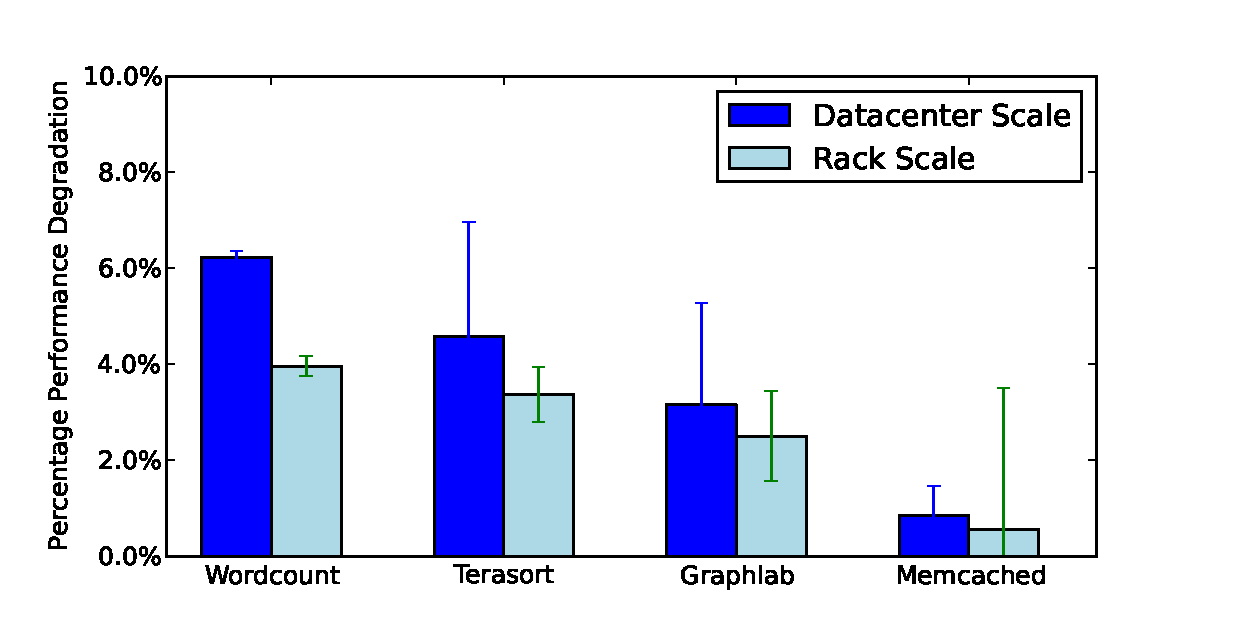
\includegraphics[width = 3in]{img/slowdown.eps} 
  \caption{\small{Application layer slowdown for each of the four applications at rack-scale and datacenter scale after injecting pFabric's FCT. The average application layer slowdown due to network effects is at most 6.2\%.}}
  \label{fig:appfabric}
\end{figure}
%

%Overall, we conclude that existing protocols should be sufficient to handle disaggregated traffic.

%
% \begin{figure}
% 	\centering
% 	\begin{tikzpicture}[xscale=0.6, yscale=0.35]

% 	\draw[thick, fill=white] (-8, 5) rectangle (-5, 9); 
% 	\draw[thick, fill=white] (-8, 9.75) rectangle (-5, 11.25); 
% 	\draw[thick, fill=white] (-8, 12) rectangle (-5, 14); 
% 	\draw (-6.5, 8.5) node {\small{Network}};
% 	\draw (-6.5, 7.5) node {\small{Simulator}};
% 	\draw (-6.5, 6.5) node {\small{(Individual}};
% 	\draw (-6.5, 5.5) node {\small{Flow delays)}};
% 	\draw (-6.5, 10.5) node {\small{Scale up}};
% 	\draw (-6.5, 13.5) node {\small{Flows from}};
% 	\draw (-6.5, 12.5) node {\small{Step (a)}};
% 	\draw[thick, black, ->] (-6.5, 12) -- (-6.5, 11.25);
% 	\draw[thick, black, ->] (-6.5, 9.75) -- (-6.5, 9);
% 	\draw[thick, black, -] (-5, 7) -- (-4.5, 7);
% 	\draw[thick, black, -] (-4.5, 7) -- (-4.5, 10.5);
% 	\draw[thick, black, ->] (-4.5, 10.5) -- (-3.75, 10.5);

% 	\draw[thick, fill=white] (-3, 5) rectangle (1, 13); 
% 	\draw[thick, fill=white] (-2, 14) rectangle (0, 12); 
% 	\draw (-1, 13) node {\small{CPU}};
% 	% \draw (-1, 10.5) node {\small{Handler}};
	
% 	\draw[thick, fill=cyan] (-3.75, 9.9) rectangle (1.75, 11.1); 
% 	\draw (-1, 10.5) node {\small{SIT (Latency Injection)}};
			
% 	\draw[thick, fill=blue] (-2.75, 7.5) rectangle (-0.75, 8.5);
% 	\draw[thick, fill=green] (-2.75, 5.5) rectangle (-0.75, 7.5);
% 	\draw (-1.75, 8) node {\small{LM}};
% %	\draw (-2.75, 7.5) -- (-0.75, 7.5);
% 	\draw (-1.75, 6.5) node {\small{RM}};
% %	\draw (-2.75, 6.5) -- (-0.75, 6.5);
% %	\draw (-1.75, 6) node {\small{K$\to$O}};

% %	\draw[thick] (-0.25, 5.5) rectangle (0.75, 8.5);
% 	\draw[thick, fill=gray] (-0.25, 8.5) rectangle (0.75, 7.5);
% 	\draw[thick, fill=gray] (-0.25, 5.5) rectangle (0.75, 6.5);
% 	\draw (0.25, 7) node {\small{$\dots$}};

% 	\draw[very thick, black, dashed, <->] (-1.5, 10) -- (-1.75, 8.5);
% 	\draw[very thick, black, dashed, <->] (-0.5, 10) -- (0.25, 8.5);
% 	\draw[very thick, black, dashed, <->] (-0.5, 10) -- (-0.45, 6);

% 	\draw[very thick, black, dashed, <->] (-1.5, 11) -- (-1.5, 12);
% 	\draw[very thick, black, dashed, <->] (-0.5, 11) -- (-0.5, 12);
% 	\draw[very thick, black, dashed, <->] (-0.5, 11) -- (-0.5, 12);

% 	\end{tikzpicture}
% 	    \caption{\small{We run real-world applications on a $5$-node Amazon EC2 cluster. To emulate end-to-end network latency, we inject artificial latencies for all ``remote memory'' and ``remote disk'' accesses and measure the impact of this latency to the application-level performance. The latencies injected for each flow are now a result of network simulation results. \rc{SIT representation imprecise}}}
% 	\label{fig:system3}
% \end{figure}
